% ------------------------------------------------------------------------------
% TYPO3 Version 9.4 - What's New (French Version)
%
% @license	Creative Commons BY-NC-SA 3.0
% @link		https://typo3.org/help/documentation/whats-new/
% @language	French
% ------------------------------------------------------------------------------

\section{Changements pour les intégrateurs}
\begin{frame}[fragile]
	\frametitle{Changements pour les intégrateurs}

	\begin{center}\huge{Chapitre 2~:}\end{center}
	\begin{center}\huge{\color{typo3darkgrey}\textbf{Changements pour les intégrateurs}}\end{center}

\end{frame}

% ------------------------------------------------------------------------------
% #85256 - Install TYPO3 on SQLite

\begin{frame}[fragile]
	\frametitle{Changements pour les intégrateurs}
	\framesubtitle{Installer TYPO3 sur SQLite (1)}

	\begin{itemize}
		\item TYPO3 supporte maintenant \href{https://www.sqlite.org}{SQLite},
			un moteur de base de données SQL open source léger et indépendant
		\item Il est possible de sélectionner SQLite pendant le processus d'installation web,
			si le module PHP «~pdo\_sqlite~» est installé et activé~:
	\end{itemize}

	\begin{figure}
		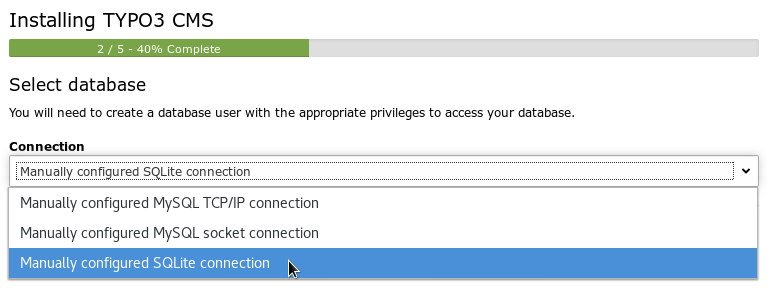
\includegraphics[width=0.65\linewidth]{ChangesForIntegrators/85256-InstallTYPO3OnSQLite.png}
	\end{figure}

\end{frame}

% ------------------------------------------------------------------------------
% #85256 - Install TYPO3 on SQLite

\begin{frame}[fragile]
	\frametitle{Changements pour les intégrateurs}
	\framesubtitle{Installer TYPO3 sur SQLite (2)}

	\begin{itemize}
		\item La base est stocké dans un fichier seul, ce qui signifie que les
			instances de TYPO3 peuvent s'exécuter avec seulement PHP, incluant le stockage
		\item L'utilisation de SQLite fait sens pour les petits sites TYPO3 et
			pour les instances de développement et test, entre autres.
		\item Les administrateurs système doivent prendre les mesures appropriées
			pour protéger le fichier \texttt{*.sqlite} d'accès non autorisés, lorsque
			celui-ci est placé dans le conteneur Web (dépendant du type d'installation)
	\end{itemize}

\end{frame}

% ------------------------------------------------------------------------------
% #85947 - Page based URL handling

\begin{frame}[fragile]
	\frametitle{Changements pour les intégrateurs}
	\framesubtitle{Gestion des URL des pages}

	\begin{itemize}
		\item Tous les liens générés par le backend et frontend utilisent ce champ,
			si défini
		\item La gestion des URL des page nécessite une configuration de site
	\end{itemize}

	\begin{figure}
		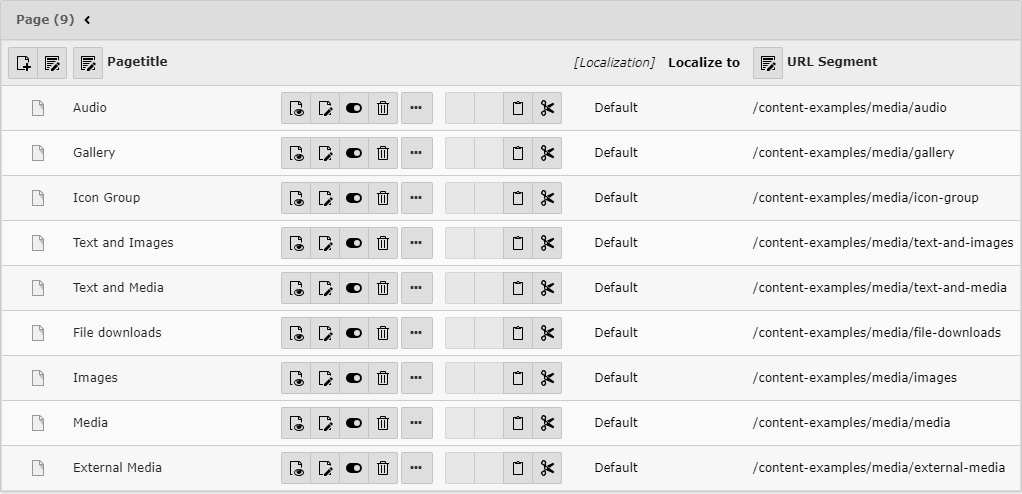
\includegraphics[width=0.7\linewidth]{ChangesForIntegrators/xxxxx-UrlSegments.png}
	\end{figure}

\end{frame}

% ------------------------------------------------------------------------------
% #84729 - New TCA type "slug"

\begin{frame}[fragile]
	\frametitle{Changements pour les intégrateurs}
	\framesubtitle{Gestion des URL des pages}

	% decrease font size for code listing
	\lstset{basicstyle=\smaller\ttfamily}

	\begin{itemize}
		\item Le type de champ TCA \texttt{slug} est ajouté
		\item Il défini les parties du chemin de l'URL à générer et
			résoud les URLs

		\begin{lstlisting}
'type' => 'slug',
  'config' => [
    'generatorOptions' => [
      'fields' => ['title', 'nav_title'],
      'fieldSeparator' => '/',
      'prefixParentPageSlug' => true
    ]
    'fallbackCharacter' => '-',
    'eval' => 'uniqueInSite'
  ]
		\end{lstlisting}
	\end{itemize}

\end{frame}

% ------------------------------------------------------------------------------
% #44297 - Interval presets for cron command of scheduler task

\begin{frame}[fragile]
	\frametitle{Changements pour les intégrateurs}
	\framesubtitle{Planificateur de tâches}

	\begin{itemize}
		\item Les valeurs prédéfinies sont ajoutées pour la planification. Les valeurs prédéfinies~:

			\begin{itemize}
				\item \texttt{0 9,15 * * 1-5}\tabto{3.8cm}(Lun. à Vend. à 9:00 et 15:00)
				\item \texttt{0 */2 * * *}\tabto{3.8cm}(toutes les 2 heures)
				\item \texttt{*/20 * * * *}\tabto{3.8cm}(toutes les 20 minutes)
				\item \texttt{0 7 * * 2}\tabto{3.8cm}(chaque mardi à 7:00)
			\end{itemize}

	\end{itemize}

	\begin{figure}
		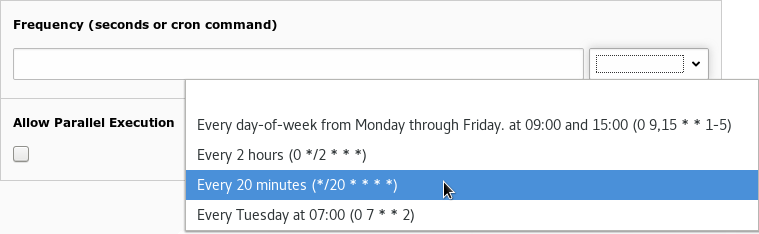
\includegraphics[width=0.80\linewidth]{ChangesForIntegrators/44297-IntervalPresetsInSchedulerTask.png}
	\end{figure}

\end{frame}

% ------------------------------------------------------------------------------
% #83476 - Load merged JS files asynchronous
% #85146 - Read environment variables in TypoScript

\begin{frame}[fragile]
	\frametitle{Changements pour les intégrateurs}
	\framesubtitle{Changements/Améliorations TypoScript (1)}

	% decrease font size for code listing
	\lstset{basicstyle=\smaller\ttfamily}

	\begin{itemize}
		\item L'attribute \texttt{async} est ajouté à la balise script des fichiers JS
			concaténés, si tous les fichiers possèdent cet attribut d'activé
			en TypoScript~:

			\begin{lstlisting}
config.concatenateJs = 1
page = PAGE
page.includeJSFooter {
  test = path/to/file.js
  test.async = 1
}
			\end{lstlisting}

		\item Les variables d'environnement peuvent être lues en TypoScript~:

			\begin{lstlisting}
# Define default value
myConstant = defaultValue
# Enable overriding by environment variable
myConstant := getEnv(MYCONSTANT)
			\end{lstlisting}

	\end{itemize}

\end{frame}

% ------------------------------------------------------------------------------
% #85550 - Add context check for TypoScript

\begin{frame}[fragile]
	\frametitle{Changements pour les intégrateurs}
	\framesubtitle{Changements/Améliorations TypoScript (2)}

	% decrease font size for code listing
	\lstset{basicstyle=\smaller\ttfamily}

	\begin{itemize}
		\item La nouvelle Context API (voir section «~Changements pour les développeurs~»)
			est aussi accessible en TypoScript pour les intégrateurs

		\item Par exemple~:

			\begin{lstlisting}
10 = TEXT
10.data = context:workspace:id
			\end{lstlisting}

		\item La syntaxe est~: \texttt{context:[aspect]:[propriété]}

		\item Les tableaux sont automatiquement convertis en listes séparées par des virgules\newline
			\smaller(idéal pour lire les informations d'appartenances aux groupes par exemple)\normalsize

	\end{itemize}

\end{frame}

% ------------------------------------------------------------------------------
% #86057 - Improved typolink / URL link generation

\begin{frame}[fragile]
	\frametitle{Changements pour les intégrateurs}
	\framesubtitle{Changements/Améliorations TypoScript (3)}

	% decrease font size for code listing
	\lstset{basicstyle=\smaller\ttfamily}

	\begin{itemize}
		\item Avec la nouvelle gestion de sites, le paramètre \texttt{GET}
			standard de fait «~L~» est devenu obsolète
		\item Le paramètre \texttt{typolink.language} est introduit

			\begin{lstlisting}
page.10 = TEXT
page.10.value = Link to the page with the ID in the current language
page.10.typolink.parameter = 23
page.20 = TEXT
page.20.value = Link to the page with the ID in the language 3
page.20.typolink.parameter = 23
page.20.typolink.language = 3
			\end{lstlisting}

	\end{itemize}

\end{frame}

% ------------------------------------------------------------------------------
% #85196 - Unify simulate user settings for Backend admins

\begin{frame}[fragile]
	\frametitle{Changements pour les intégrateurs}
	\framesubtitle{Simuler l'utilisateur dans les options d'utilisateur BE}

	\begin{itemize}
		\item Les administrateurs avaient la possibilité de basculer vers un autre
			utilisateur («~User Settings → Simulate backend user~»)
		\item Ceci est retiré
	\end{itemize}

	\begin{figure}
		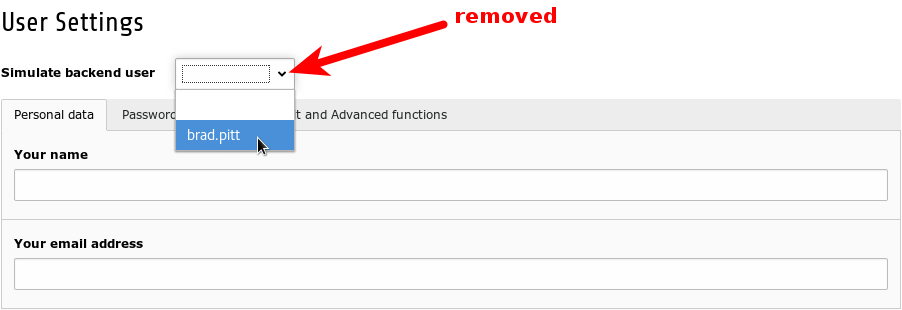
\includegraphics[width=0.80\linewidth]{ChangesForIntegrators/85196-SimulateUserRemovedForAdmins.png}
	\end{figure}

\end{frame}

% ------------------------------------------------------------------------------
% #84133 - Introduce variants

\begin{frame}[fragile]
	\frametitle{Changements pour les intégrateurs}
	\framesubtitle{Alternatives conditionnelles dans \texttt{EXT:form} (1)}

	\begin{itemize}
		\item Nouvelle fonctionnalité pour l'extension «~Forms~»~: \textit{conditional variants}
		\item Les alternatives peuvent contenir des conditions et permettent de modifier les
			propriétés des éléments de formulaire
		\item Ainsi, il est possible de manipuler les valeurs, les options des validateurs et
			des finaliseurs, etc. des éléments en fonction de conditions

	\end{itemize}

\end{frame}

% ------------------------------------------------------------------------------
% #84133 - Introduce variants

\begin{frame}[fragile]
	\frametitle{Changements pour les intégrateurs}
	\framesubtitle{Alternatives conditionnelles dans \texttt{EXT:form} (2)}

	\begin{itemize}
		\item Des cas d'usage typiques sont par exemple~:

			\begin{itemize}
				\item Traduire les valeurs d'un élément en fonction de la langue actuelle.
				\item Définir et retirer des validateurs en fonction des valeurs d'autres
					élément du formulaire.
				\item Définir la valeur du finaliseur en fonction de la valeur d'un élément.
				\item Cacher un élément dans certains finaliseurs et sur la page de résumé.
				\item Cacher complètement une page du tunnel en fonction de la valeur d'un élément.
				\item etc.
			\end{itemize}

		\item La \href{https://docs.typo3.org/typo3cms/extensions/form}{documentation officielle}
			contient plus d'information ainsi que des exemples.

	\end{itemize}

\end{frame}

% ------------------------------------------------------------------------------
% #85355 - Support basic HTML5 fields in FormEngine

\begin{frame}[fragile]
	\frametitle{Changements pour les intégrateurs}
	\framesubtitle{Validation HTML5 des champs du backend}

	\begin{itemize}
		\item Dans le backend, la FormEngine utilise maintenant les types de champs
		    et attributs spécifiques de HTML5
		\item Ceci inclus les courriels, les nombres avec la configuration de
			l'intervalle, par exemple
		\item Les attributs des balises sont basés sur la configuration \texttt{eval} en TCA
		\item Potentiellement, cette fonction rendera le traitement en JavaScript obsolète
			au long terme
	\end{itemize}

\end{frame}

% ------------------------------------------------------------------------------
% #86001 - Regular Workspace cleanup tasks available via CLI commands

\begin{frame}[fragile]
	\frametitle{Changements pour les intégrateurs}
	\framesubtitle{Commandes CLI des espaces de travail}

	% decrease font size for code listing
	\lstset{basicstyle=\small\ttfamily}

	\begin{itemize}
		\item Deux nouvelles commandes symfony pour des tâches régulières~:

			\begin{itemize}

				\item \texttt{workspace:autopublish}\newline
					Vérifie les espaces de travail avec l'auto-publication
					configurée et effectue le processus de publication/échange.
					\newline

				\item \texttt{cleanup:previewlinks}\newline
					Nettoie les liens de prévisualisations présents
					dans sys\_preview de la base.

			\end{itemize}

		\item Exécution en ligne de commande, par exemple~:

			\begin{lstlisting}
$ typo3/sysext/core/bin/typo3 workspace:autopublish
			\end{lstlisting}

	\end{itemize}

\end{frame}

% ------------------------------------------------------------------------------
% #81430 - Improve TS Template module information on root level list

\begin{frame}[fragile]
	\frametitle{Changements pour les intégrateurs}
	\framesubtitle{Module d'information TypoScript}

	\begin{itemize}
		\item Aperçu des gabaris TypoScript sur la page racine retravaillé
		\item Le rendu passe maintenant par Fluid
		\item Les informations affichées incluent le nom de la page,
			le nom du gabarit (avec le lien pour l'éditer), l'état (icône),
			si racine ou d'extension

	\end{itemize}

	\begin{figure}
		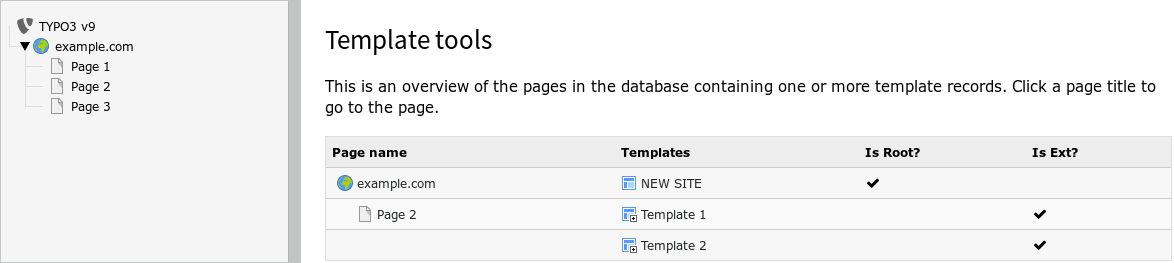
\includegraphics[width=0.80\linewidth]{ChangesForIntegrators/81430-TypoScriptModuleInformation.png}
	\end{figure}

\end{frame}

% ------------------------------------------------------------------------------
% #85393 - Only import extensions from 2015+ into EM

\begin{frame}[fragile]
	\frametitle{Changements pour les intégrateurs}
	\framesubtitle{Gestionnaire d'extensions}

	\begin{itemize}
		\item Les extensions plus anciennes que le 10 novembre 2015 (TYPO3 v7 LTS)
			sont exclues de l'import de la liste d'extensions
		\item Ceci réduit la taille de la table en base de 75\% environ
	\end{itemize}

\end{frame}

% ------------------------------------------------------------------------------
